\documentclass[letterpaper, 12pt]{article}
\usepackage[margin=1in]{geometry}
\usepackage{amsmath}
\usepackage{amssymb}
\usepackage{fancyhdr}
\usepackage{graphicx}
\usepackage{xcolor}
\usepackage{hyperref}
\usepackage{float}

\pagestyle{fancy}
\fancyhf{}

\rhead{
    Shengdong Li
    Calc 1
}
\rfoot{
    Page \thepage
}

\usepackage{indentfirst}
\setlength{\parindent}{2em}

\begin{document}
\title{In Conclusion}
\author{by Shengdong Li}
\date{26 April 2020}
\maketitle

\section{Intro}
First I'll check my work in my initial post using the disk/washer method.

\section{Solution}
\begin{align}
    \intertext{First put equations in terms of $y$}
    y&=x^{2}\\
    &=x=\sqrt{y}\\
    y&=\sqrt{x}\\
    &=x=y^{2}
    \intertext{Graph.}
\end{align}
\begin{figure}[H]
    \begin{center}
        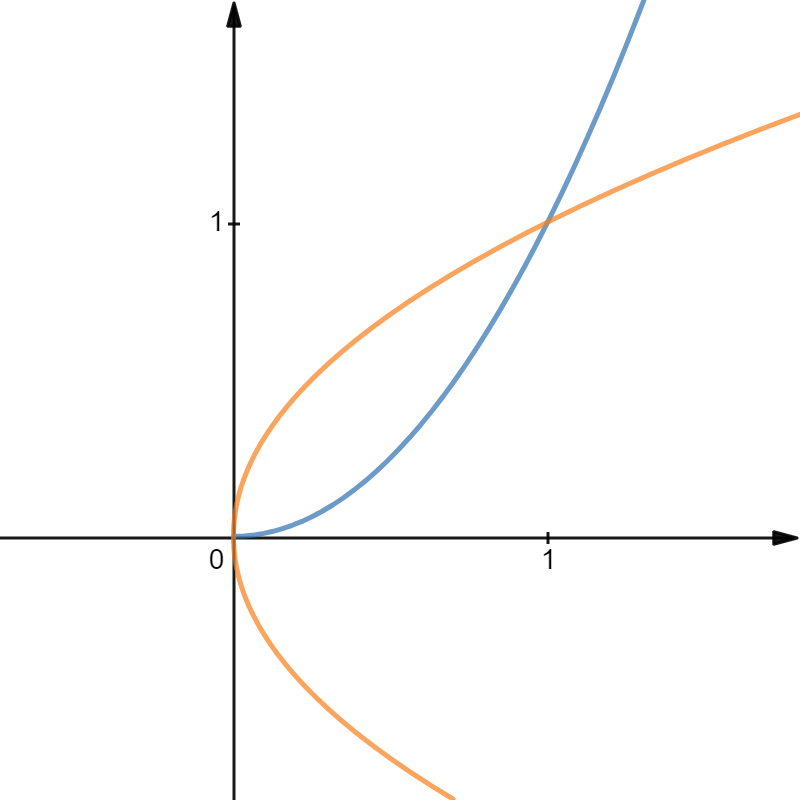
\includegraphics[scale=.2]{2FuncConc.png}
        \caption{\textit{Graph of (Orange) $x=y^2$ and (Blue) $x=\sqrt{y}$.} Desmos link \href{https://www.desmos.com/calculator/vfywew4f0z}{\textcolor{blue}{here}}.}
    \end{center}
\end{figure}
\begin{align}
    \intertext{Define the inner and outer functions from the graph}
    \text{Outer: }                                                                                     x &= \sqrt{y}                                                                                                                                    \\
    \text{Inner: }                                                                                     x &= y^2
    \intertext{Define the ranges. From the graph it is apparent that the bottom bound is $0$ and the upper bound is $1$}
    a                                                                                               & = 0                                                                                                                                       \\
    b                                                                                               & = 1
    \intertext{Plugin to the disk/washer equation to calculate volume using circular cross-sections perpendicular to the $y$-axis}
    \pi\int_{a}^{b}\left(\left(f\left(y\right)\right)^{2}-\left(g\left(y\right)\right)^{2}\right)dy & =\pi\int_{0}^{1}\left(\left(\sqrt{y}\right)^{2}-\left(y^{2}\right)^{2}\right)dy                                                                   \\
                                                                                                    & =\pi\int_{0}^{1}\left(y-y^{4}\right)dy                                                                                                            \\
                                                                                                    & =\pi\left(\frac{y^{2}}{2}-\frac{y^{5}}{5}\right)\Big|_{0}^{1}                                                                                     \\
                                                                                                    & =\pi\left(\frac{\left(1\right)^{2}}{2}-\frac{\left(1\right)^{5}}{5}-\left(\frac{\left(0\right)^{2}}{2}-\frac{\left(0\right)^{5}}{5}\right)\right) \\
                                                                                                    & =\pi\left(\frac{1}{2}-\frac{1}{5}\right)                                                                                                          \\
                                                                                                    & =\frac{3\pi}{10}                                                                                                                                  \\
                                                                                                    & \approx\boxed{.942}
\end{align}
\section{A discussion of the shell method vs. disk/washer method}
Looking at the two methods, one clear difference is that the disk/washer method is based fully off the distance between two equations with respect to the axis the area is being rotated around. Therefore, you must set equations rotated around the $x$-axis in terms of $x$ to solve for $y$ and equations rotated around the $y$-axis in terms of $y$ to solve for $x$; Equations are \textbf{perpendicular} to the axis. However, the shell method is based off the height of the cylinder. Therefore, it is actually in \textbf{parallels} with the axis that it is being rotated around. I feel that both methods are situtationally good: if you were given equations in terms of $y$ rotated around the $x$ axis, then shell would definitely take less time and less steps than the disk/washer method, but if if it was in terms of $x$ then disk/washer instead would be the more efficient method.
\end{document}